\documentclass[%
 reprint,
%superscriptaddress,
%groupedaddress,
%unsortedaddress,
%runinaddress,
%frontmatterverbose, 
%preprint,
%preprintnumbers,
%nofootinbib,
%nobibnotes,
%bibnotes,
 amsmath,amssymb,
 aps,
%pra,
%prb,
%rmp,
%prstab,
%prstper,
%floatfix,
]{revtex4-2}
\usepackage{multirow}
\usepackage{graphicx}% Include figure files
\usepackage{dcolumn}% Align table columns on decimal point
\usepackage{bm}% bold math
%\usepackage{hyperref}% add hypertext capabilities
%\usepackage[mathlines]{lineno}% Enable numbering of text and display math
%\linenumbers\relax % Commence numbering lines

%\usepackage[showframe,%Uncomment any one of the following lines to test 
%%scale=0.7, marginratio={1:1, 2:3}, ignoreall,% default settings
%%text={7in,10in},centering,
%%margin=1.5in,
%%total={6.5in,8.75in}, top=1.2in, left=0.9in, includefoot,
%%height=10in,a5paper,hmargin={3cm,0.8in},
%]{geometry}
\usepackage[utf8x]{inputenc} % Включаем поддержку UTF8  
\usepackage[russian]{babel}  % Включаем пакет для поддержки русского языка 
\usepackage[normalem]{ulem}  % для зачекивания текста

\usepackage[noend]{algorithmic}
\def\algorithmicrequire{\textbf{Вход:}}
\def\algorithmicensure{\textbf{Выход:}}
\def\algorithmicif{\textbf{если}}
\def\algorithmicthen{\textbf{то}}
\def\algorithmicelse{\textbf{иначе}}
\def\algorithmicelsif{\textbf{иначе если}}
\def\algorithmicfor{\textbf{для}}
\def\algorithmicforall{\textbf{для всех}}
\def\algorithmicdo{}
\def\algorithmicwhile{\textbf{пока}}
\def\algorithmicrepeat{\textbf{повторять}}
\def\algorithmicuntil{\textbf{пока}}
\def\algorithmicloop{\textbf{цикл}}
% переопределение стиля комментариев
\def\algorithmiccomment#1{\quad// {\sl #1}}
\usepackage{caption}

\usepackage{subcaption}
\usepackage{multirow}
\usepackage[table,xcdraw]{xcolor}
\begin{document}



\title{Лабораторная работа 1.3\\Изучение рассеяния медленных электронов на атомах (эффект Рамзауэра)}% Force line breaks with \\



\author{Батарин Егор Владиславович}
\affiliation{%
 Студент 3 курса РТ\\
}%

\collaboration{Московский физико-технический институт}%\noaffiliation

\date{\today}% It is always \today, today,
             %  but any date may be explicitly specified
             

\begin{abstract}
Исследуется энергетическая зависимость вероятности рассеяния электронов атомами ксенона, определяются энергии электронов, при которых наблюдается "просветление" ксенона, и оценивается размер его внешней электронной оболочки.  
\begin{description}
\item[Оборудование]
Тиратрон ТГ3-01/1.3Б, осциллограф, стабилизированный БНС.
\end{description}
\end{abstract}

%\keywords{Suggested keywords}%Use showkeys class option if keyword
                              %display desired
\maketitle

%\tableofcontents

\section{Теоретическая часть.}

Вводится понятие эффективного сечения реакции $\sigma = \frac{N}{nv}$, характеризующая вероятность перехода системы из двух сталкивающихся частич в определенное состояние, в результате их рассеяния. Знаменатель равен плотности потока всех рассеиваемых частиц, числитель - число таких переходов.
К. Рамзауэр исследовал зависимость поперечных сечений упрогого рассеяния электронов (с энергией до 10 ЭВ) на атомах аргона. В результате этих исследований было обнаружено явление, получившее название \textit{эффекта Рамзауэра}.

С точки зрения квантовой теории атом по отношению к электронной волне ведет себя как преломляющая среда с относительным показателем преломления
\begin{equation*}
n = \frac{\lambda}{\lambda^\prime} = \sqrt{1-\frac{U}{E}},
\end{equation*}
где $U$, $E$ -- соответственно потенциальная и полная энергии электрона внутри атома.

Будем считать, что электрон рассеивается на одномерной прямоугольной потенциальной яме конечной глубины. Такая модель является хорошим приближением для атомов тяжелых инертных газов, отличающихся наиболее компактной структурой и резкой внешней границей. Решение задачи о прохождении частицы с энергией $E$ над потенциальной ямой шириной $l$ и глубиной $U_0$ не составит труда найти из уравнения Шредингера:\\
\begin{equation*}
\psi^{\prime\prime}+k^2\psi=0, \ \text{где}\
k^2 =\begin{cases}
2mE/\hbar^2 & x<0, x>l\\
(2mE+U_0)/\hbar^2 & 0<x<l
\end{cases}.
\end{equation*}
Коэффициент прохождения равен отношению квадратов амплитуд прошедшей и падающей волн и определяется выражением:
\begin{equation*}
\frac{1}{D} = 1 + \frac{U_0^2}{4E(E+U_0)}\sin^2(k_2l).
\end{equation*}
Минимум последнего выражения отвечает квантовому аналогу просветления оптики, так как при выполнении условия
\begin{equation*}
\tag{$\star$}
\label{eq:uslovie}
\sqrt{\frac{2m(E+U_0)}{\hbar^2}}l = \pi n, \ n\in\mathbb{N},
\end{equation*}
коэффициент прохождения частицы над ямой становится равным единице, то есть достигает своего максимального значения.
Отметим, что условие~(\ref{eq:uslovie}) легко получить, рассматривая интерференцию электронов волн де Бройля в атоме:\\
\begin{itemize}
	\item
	Условие первого интерференционного максимума:
	\begin{equation}
	\label{eq:1}
	2l = \frac{h}{\sqrt{2m(E_1+U_0)}}.
	\end{equation}
	\item
	Условие первого интерференционного минимума:
	\begin{equation}
	\label{eq:2}
	2l =\frac{3}{2} \frac{h}{\sqrt{2m(E_1+U_0)}}.
	\end{equation}			
\end{itemize}

Решая совместно уравнения~(\ref{eq:1}, \ref{eq:2}) можно получить:
\begin{equation}
\label{eq:l}
l = \frac{h\sqrt{5}}{\sqrt{32m(E_2-E_1)}}.
\end{equation}
Понятно, что энергии $E_1$ и $E_2$ соответствуют энергиям электронов, прошедших разность потенциалов $V_1$ и $V_2$, то есть $E_1 = eV_1$ и $E_2 = eV_2$. 

По измеренным величинам $E_1$ и $E_2$, используя формулы~(\ref{eq:1}, \ref{eq:2}), можно рассчитать эффективную глубину потенциальной ямы атома:
\begin{equation}
\label{eq:U_0}
U_0 = \frac{4}{5}E_2 - \frac{9}{5}E_1
\end{equation}

Согласно квантовой механике зависимость вероятности рассеяния электрона от его энергии можно определить из соотношения:
\begin{equation}
\label{eq:w}
w(U) = -\frac{1}{C}\ln \frac{I(U)}{I_0},
\end{equation}
где $I_0$ -- ток катода, а $C$ -- некторая постоянная.

\section{Методика измерений}

В эксперименте будем исследовать ВАХ двумя методами: статическими и динамическим. В статическом методе будем снимать показания напряжения с вольтметра и амперметра при различных значениях напряжения анода, в динамическом методе сразу используем картину на осциллографе. 


\section{Основные результаты и их обсуждение.}
Имеем 2 таблицы основным результатов.

\begin{figure*}[h!]
	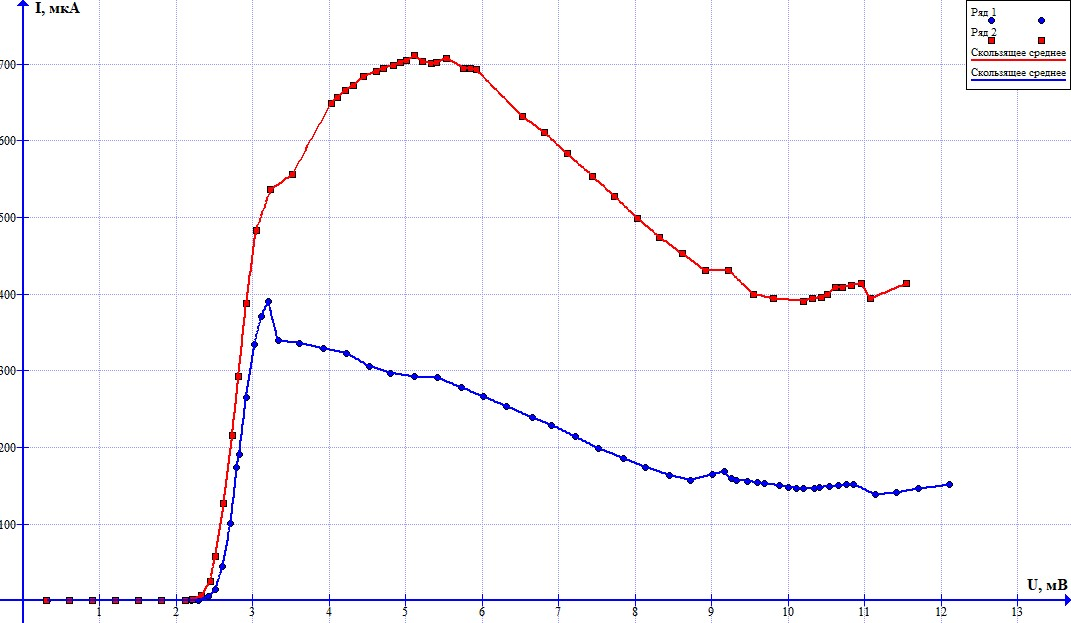
\includegraphics[scale=0.5]{1.jpg}
\end{figure*}
\begin{figure*}[h!]
	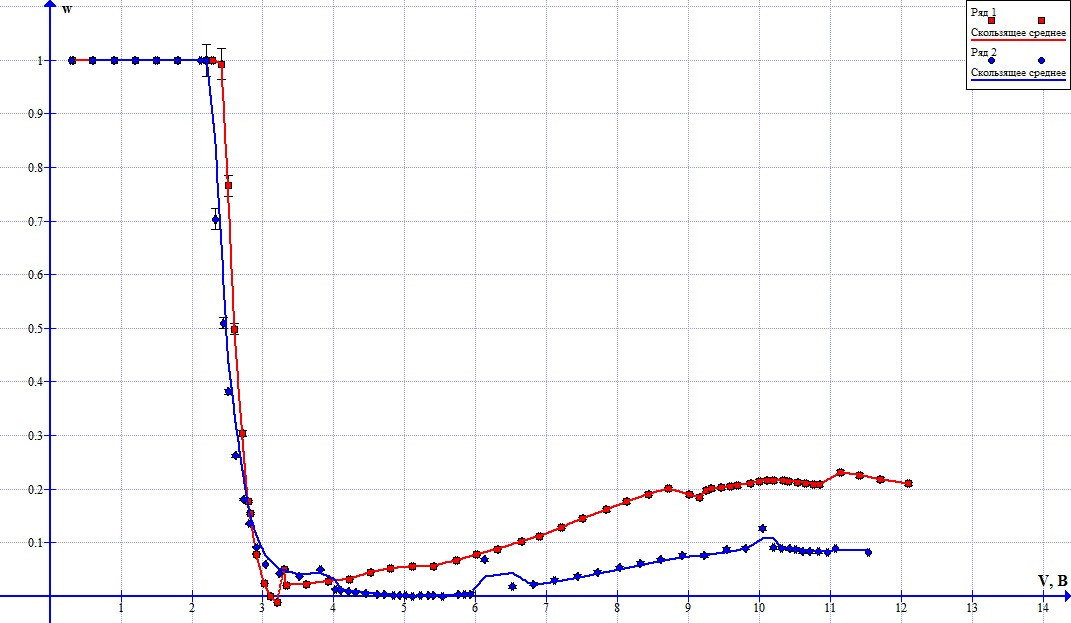
\includegraphics[scale=0.4]{2.jpg}
\end{figure*}

\begin{table}[h!]
	\begin{tabular}{|l|l|l|l|l|}
		\hline
		\multicolumn{5}{|c|}{\multirow{2}{*}{ВАХ и $\omega$ при $U_\text{н} = 2.63$}} \\
		\multicolumn{5}{|c|}{}                                       \\ \hline
		$V_i$, мВ    & $V$, В     & $I$, мкА    & $\omega$           & $\delta\omega$          \\ \hline
		0         & 0.32     & 0         & 1           & 0           \\ \hline
		0         & 0.6      & 0         & 1           & 0           \\ \hline
		0         & 0.9      & 0         & 1           & 0           \\ \hline
		0         & 1.2      & 0         & 1           & 0           \\ \hline
		0         & 1.5      & 0         & 1           & 0           \\ \hline
		0         & 1.8      & 0         & 1           & 0           \\ \hline
		0         & 2.2      & 0         & 1           & 0           \\ \hline
		0         & 2.29     & 0         & 1           & 0           \\ \hline
		0.53      & 2.42     & 5.3       & 0.992639    & 0.029633    \\ \hline
		1.4       & 2.51     & 14        & 0.765688    & 0.019382    \\ \hline
		4.4       & 2.6      & 44        & 0.498134    & 0.009944    \\ \hline
		10.1      & 2.71     & 101       & 0.303991    & 0.004888    \\ \hline
		17.4      & 2.79     & 174       & 0.176903    & 0.002395    \\ \hline
		19.1      & 2.82     & 191       & 0.155124    & 0.002033    \\ \hline
		26.5      & 2.91     & 265       & 0.078615    & 0.00091     \\ \hline
		33.5      & 3.02     & 335       & 0.023848    & 0.00025     \\ \hline
		37.1      & 3.11     & 371       & 0           & 0           \\ \hline
		39        & 3.2      & 390       & -0.01167    & -0.00011    \\ \hline
		29.8      & 3.3      & 298       & 0.051194    & 0.000564    \\ \hline
		33.9      & 3.33     & 339       & 0.021075    & 0.00022     \\ \hline
		33.6      & 3.61     & 336       & 0.023152    & 0.000242    \\ \hline
		32.9      & 3.92     & 329       & 0.028071    & 0.000296    \\ \hline
		32.3      & 4.22     & 323       & 0.032371    & 0.000345    \\ \hline
		30.6      & 4.52     & 306       & 0.045004    & 0.000491    \\ \hline
		29.7      & 4.8      & 297       & 0.051979    & 0.000574    \\ \hline
		29.2      & 5.11     & 292       & 0.055946    & 0.000622    \\ \hline
		29.1      & 5.41     & 291       & 0.056747    & 0.000632    \\ \hline
		27.8      & 5.73     & 278       & 0.067425    & 0.000765    \\ \hline
		26.6      & 6.01     & 266       & 0.077735    & 0.000898    \\ \hline
		25.4      & 6.31     & 254       & 0.088521    & 0.001042    \\ \hline
		23.9      & 6.65     & 239       & 0.102743    & 0.001239    \\ \hline
		22.9      & 6.9      & 229       & 0.112729    & 0.001381    \\ \hline
		21.4      & 7.21     & 214       & 0.128557    & 0.001616    \\ \hline
		19.9      & 7.51     & 199       & 0.145537    & 0.001879    \\ \hline
		18.6      & 7.84     & 186       & 0.161321    & 0.002134    \\ \hline
		17.43     & 8.13     & 174.3     & 0.176501    & 0.002388    \\ \hline
		16.4      & 8.44     & 164       & 0.190733    & 0.002635    \\ \hline
		15.7      & 8.72     & 157       & 0.200924    & 0.002817    \\ \hline
		16.5      & 9.01     & 165       & 0.189312    & 0.00261     \\ \hline
		16.8      & 9.16     & 168       & 0.185102    & 0.002536    \\ \hline
		15.9      & 9.25     & 159       & 0.197967    & 0.002763    \\ \hline
		15.7      & 9.32     & 157       & 0.200924    & 0.002817    \\ \hline
		15.6      & 9.46     & 156       & 0.202417    & 0.002844    \\ \hline
		15.4      & 9.59     & 154       & 0.205432    & 0.002898    \\ \hline
		15.3      & 9.69     & 153       & 0.206954    & 0.002926    \\ \hline
		15        & 9.88     & 150       & 0.211581    & 0.003011    \\ \hline
		14.8      & 10       & 148       & 0.214717    & 0.003069    \\ \hline
		14.7      & 10.11    & 147       & 0.216301    & 0.003099    \\ \hline
		14.7      & 10.2     & 147       & 0.216301    & 0.003099    \\ \hline
		14.7      & 10.34    & 147       & 0.216301    & 0.003099    \\ \hline
		14.8      & 10.41    & 148       & 0.214717    & 0.003069    \\ \hline
		14.9      & 10.54    & 149       & 0.213144    & 0.00304     \\ \hline
		15        & 10.65    & 150       & 0.211581    & 0.003011    \\ \hline
		15.15     & 10.76    & 151.5     & 0.209256    & 0.002968    \\ \hline
		15.2      & 10.85    & 152       & 0.208486    & 0.002954    \\ \hline
		13.8      & 11.14    & 138       & 0.231063    & 0.003378    \\ \hline
		14.1      & 11.41    & 141       & 0.226038    & 0.003282    \\ \hline
		14.58     & 11.7     & 145.8     & 0.218216    & 0.003135    \\ \hline
		15.1      & 12.1     & 151       & 0.210029    & 0.002983    \\ \hline
	\end{tabular}
\end{table}

\begin{table}[h!]
	\begin{tabular}{|l|l|l|l|l|}
		\hline
		\multicolumn{5}{|c|}{\multirow{2}{*}{ВАХ и $\omega$ при $U_\text{н} = 2.89$}} \\
		\multicolumn{5}{|c|}{}                                       \\ \hline
		$V_i$, мВ    & $V$, В     & $I$, мкА    & $\omega$          & $\delta\omega$          \\ \hline
		0         & 0.3      & 0         & 1           & 0           \\ \hline
		0         & 0.6      & 0         & 1           & 0           \\ \hline
		0         & 0.9      & 0         & 1           & 0           \\ \hline
		0         & 1.2      & 0         & 1           & 0           \\ \hline
		0         & 1.5      & 0         & 1           & 0           \\ \hline
		0         & 1.8      & 0         & 1           & 0           \\ \hline
		0         & 2.12     & 0         & 1           & 0           \\ \hline
		0.1       & 2.21     & 1         & 0.999494    & 0.029633    \\ \hline
		0.7       & 2.33     & 7         & 0.703312    & 0.019382    \\ \hline
		2.5       & 2.44     & 25        & 0.509558    & 0.009944    \\ \hline
		5.8       & 2.51     & 58        & 0.381466    & 0.004888    \\ \hline
		12.7      & 2.62     & 127       & 0.262174    & 0.002395    \\ \hline
		21.6      & 2.73     & 216       & 0.181339    & 0.002033    \\ \hline
		29.2      & 2.81     & 292       & 0.135452    & 0.00091     \\ \hline
		38.8      & 2.91     & 388       & 0.092187    & 0.00025     \\ \hline
		48.3      & 3.04     & 483       & 0.058852    & 0           \\ \hline
		53.6      & 3.23     & 536       & 0.043004    & -0.00011    \\ \hline
		55.6      & 3.51     & 556       & 0.037428    & 0.000564    \\ \hline
		51.4      & 3.81     & 514       & 0.049383    & 0.00022     \\ \hline
		64.9      & 4.02     & 649       & 0.013887    & 0.000242    \\ \hline
		65.7      & 4.1      & 657       & 0.012023    & 0.000296    \\ \hline
		66.6      & 4.21     & 666       & 0.009952    & 0.000345    \\ \hline
		67.3      & 4.31     & 673       & 0.00836     & 0.000491    \\ \hline
		68.4      & 4.45     & 684       & 0.005893    & 0.000574    \\ \hline
		69.1      & 4.61     & 691       & 0.004343    & 0.000622    \\ \hline
		69.5      & 4.71     & 695       & 0.003464    & 0.000632    \\ \hline
		69.9      & 4.84     & 699       & 0.002591    & 0.000765    \\ \hline
		70.2      & 4.93     & 702       & 0.001939    & 0.000898    \\ \hline
		70.5      & 5.01     & 705       & 0.00129     & 0.001042    \\ \hline
		71.1      & 5.11     & 711       & 0           & 0.001239    \\ \hline
		70.4      & 5.22     & 704       & 0.001506    & 0.001381    \\ \hline
		70.1      & 5.33     & 701       & 0.002156    & 0.001616    \\ \hline
		70.2      & 5.4      & 702       & 0.001939    & 0.001879    \\ \hline
		70.8      & 5.53     & 708       & 0.000644    & 0.002134    \\ \hline
		69.5      & 5.75     & 695       & 0.003464    & 0.002388    \\ \hline
		69.4      & 5.84     & 694       & 0.003683    & 0.002635    \\ \hline
		69.3      & 5.92     & 693       & 0.003903    & 0.002817    \\ \hline
		45.3      & 6.13     & 453       & 0.068612    & 0.00261     \\ \hline
		63.2      & 6.52     & 632       & 0.017927    & 0.002536    \\ \hline
		61.1      & 6.81     & 611       & 0.023071    & 0.002763    \\ \hline
		58.3      & 7.11     & 583       & 0.030211    & 0.002817    \\ \hline
		55.4      & 7.44     & 554       & 0.037977    & 0.002844    \\ \hline
		52.8      & 7.72     & 528       & 0.045293    & 0.002898    \\ \hline
		49.9      & 8.03     & 499       & 0.053891    & 0.002926    \\ \hline
		47.4      & 8.32     & 474       & 0.061715    & 0.003011    \\ \hline
		45.3      & 8.61     & 453       & 0.068612    & 0.003069    \\ \hline
		43.1      & 8.91     & 431       & 0.076189    & 0.003099    \\ \hline
		43.1      & 9.22     & 431       & 0.076189    & 0.003099    \\ \hline
		40        & 9.54     & 400       & 0.087551    & 0.003099    \\ \hline
		39.4      & 9.81     & 394       & 0.089851    & 0.003069    \\ \hline
		30.9      & 10.05    & 309       & 0.126839    & 0.00304     \\ \hline
		39.1      & 10.2     & 391       & 0.091014    & 0.003011    \\ \hline
		39.4      & 10.31    & 394       & 0.089851    & 0.002968    \\ \hline
		39.6      & 10.43    & 396       & 0.08908     & 0.002954    \\ \hline
		39.9      & 10.51    & 399       & 0.087932    & 0.003378    \\ \hline
		40.9      & 10.61    & 409       & 0.084164    & 0.003282    \\ \hline
		40.9      & 10.71    & 409       & 0.084164    & 0.003135    \\ \hline
		41.2      & 10.83    & 412       & 0.083052    & 0.002983    \\ \hline
		41.4      & 10.96    & 414       & 0.082315    & 0           \\ \hline
		39.4      & 11.07    & 394       & 0.089851    & 0           \\ \hline
		41.4      & 11.54    & 414       & 0.082315    & 0           \\ \hline
	\end{tabular}
\end{table}

По данным стоятся вольт-амперные характеристики для синего $U_\text{н} = 2.63$ В и красного $U_\text{н} = 2.89$ и зависимость вероятности рассеивания от напряжения.

\section{Заключение.}

Были доказаны доказаны квантовые свойства света на эффекте Рамзауэра, простроены ВАХ и зависимость вероятности рассеивания от напряжения. Выводы хорошо согласуются с теорией. 


\end{document}